\documentclass[10pt,a4paper]{article}

\usepackage[margin=1in]{geometry}
\usepackage[T1]{fontenc}
\usepackage[utf8]{inputenc}
\usepackage{amsmath,amssymb,amsthm}
\usepackage{booktabs}
\usepackage{graphicx}
\usepackage{float}
\usepackage{xcolor}
\usepackage{url}
\usepackage[expansion=false]{microtype}
\usepackage{hyperref}

\hypersetup{colorlinks=true, linkcolor=blue!50!black, citecolor=blue!50!black, urlcolor=blue!50!black}
\sloppy

\newtheorem{proposition}{Proposition}
\newtheorem{lemma}{Lemma}
\theoremstyle{remark}
\newtheorem{remark}{Remark}

\newcommand{\FF}{\mathbb{F}}
\newcommand{\ZZ}{\mathbb{Z}}
\newcommand{\QQ}{\mathbb{Q}}
\newcommand{\OO}{\mathcal{O}}
\newcommand{\End}{\operatorname{End}}
\newcommand{\Aut}{\operatorname{Aut}}
\newcommand{\code}[1]{\texttt{#1}}
% Artefact paths; robust so they can appear inside \caption.
\DeclareRobustCommand{\art}[1]{\texttt{\detokenize{#1}}}
\newcommand{\run}{\art{crypto:research/isogeny-class-rho/runs/run-20261018T0857Z}}

\title{Pollard Rho Across Isogeny Classes of Prime, Binary and Koblitz Curves:\\
  Historical Measurements and Review Limits}
\author{Anonymous}
\date{}

\begin{document}
\maketitle

\begin{abstract}
An $\FF_q$-rational isogeny of degree prime to $n$ restricts to an isomorphism of
the prime-order subgroup $\langle P\rangle$ on which an elliptic-curve
discrete-logarithm instance $Q = kP$ lives. This preserves the operation
distribution of a coupled algorithm in a unit-cost oracle model; concrete
hash-partitioned walks need separate evidence. We compare them
empirical statement about ``which curve'' can be tested: by carrying one
instance, through explicit and verified isogenies, to many curves of its class
and running the same Pollard rho on each, under a protocol frozen before the
first measurement, with negative controls (the same curve in other
coordinates or another field basis, an A/A replica), planted effects of known
size, and the structural folds a crater curve admits as positive controls. Four
classes are measured: a prime-field class of $347{,}004$ curves ($104$
measured, spread over all $12$ endomorphism-ring strata and reached through
isogenies of degree $3$ to $61$), a $j = 0$ class ($45$ curves), a class of
$327{,}080$ curves over $\FF_{2^{37}}$ ($40$ curves) and the class of the
Koblitz curve $y^2 + xy = x^3 + 1$ over $\FF_{2^{41}}$ ($708{,}153$ curves,
$11$ measured over all four strata). In $85{,}425$ solves, every one returning
the planted logarithm, the primary class-mode curve comparisons stayed within
their reported Bonferroni bands. Ancillary analyses recorded one flagged B1
generator, two flagged P1 source--target cells, one flagged P0 source--target
cell, and an all-arm B1 generator Kruskal--Wallis $p=0.039$; these exceptions
preclude a blanket statement that no test fired. The historical planted
negation fold ($0.63$ to $0.77$ of the unfolded mean,
expected $0.707$) and the $4$-adding walk ($1.27$ to $1.36$) were detected every
time. Historical structural-fold comparisons report that the
order-$6$ automorphism fold at $j = 0$ cost $0.439$ $[0.401, 0.481]$ of the plain
walk (expected $1/\sqrt{6} = 0.408$), and the Frobenius fold on the Koblitz
crater $0.155$ $[0.141, 0.170]$ (expected $1/\sqrt{41}$), $0.113$ with negation
(expected $1/\sqrt{82}$). The recorded $1.7$ to $2.2$ wall-time ratio is an
unisolated shared-VM observation, not an admitted performance result.
Every measured off-crater isogeny leads away from the curve that
has them. On the way we record that, for odd $m$, every prime dividing the
conductor of a curve over $\FF_{2^m}$ is $\pm 1 \bmod 8$. For the Koblitz curve
over $\FF_{2^{41}}$, its recorded conductor factorization
$703889=409\cdot1721$ additionally rules out smaller off-crater degrees; we
find its $409$- and $1721$-isogenies (division polynomials of degree
$83{,}640$ and $1{,}480{,}920$) in about one and five minutes each through
$\ell$-torsion abscissae in $\FF_{2^{41\cdot 204}}$ and $\FF_{2^{41\cdot 215}}$,
and we derive and verify an explicit V\'elu map on points for ordinary curves
in characteristic two. The inferential null is provisional: source review
found tied-sample statistical defects, and the shared-seed Welch design
requires a covariance assessment and corrected native reanalysis.
Native-harness admission and concrete formal-proof bridges also remain open.
This is rho against rho, not an index-calculus result or a claim about any
deployed curve. Code, historical records and raw per-solve rows are released.
\end{abstract}

\paragraph{Review status, 2026-10-19.}
The numerical tables and figures below retain the historical analysis.
Companion source review found a tied-sample KS defect: identical samples
$[1,1]$ and $[1,1]$ return $D=1$ instead of $0$. Rank-test tie corrections
and the covariance induced by shared seeds also require review. Corrected
native analysis, traceable to the frozen rows and source revision, is still
owed; no historical $p$-value or inferred null is promoted as corrected here.
Native ecbench admission and concrete Lean proof bridges remain open.
The versioned review and proof map live beside this manuscript.

\begin{figure}[H]
\centering
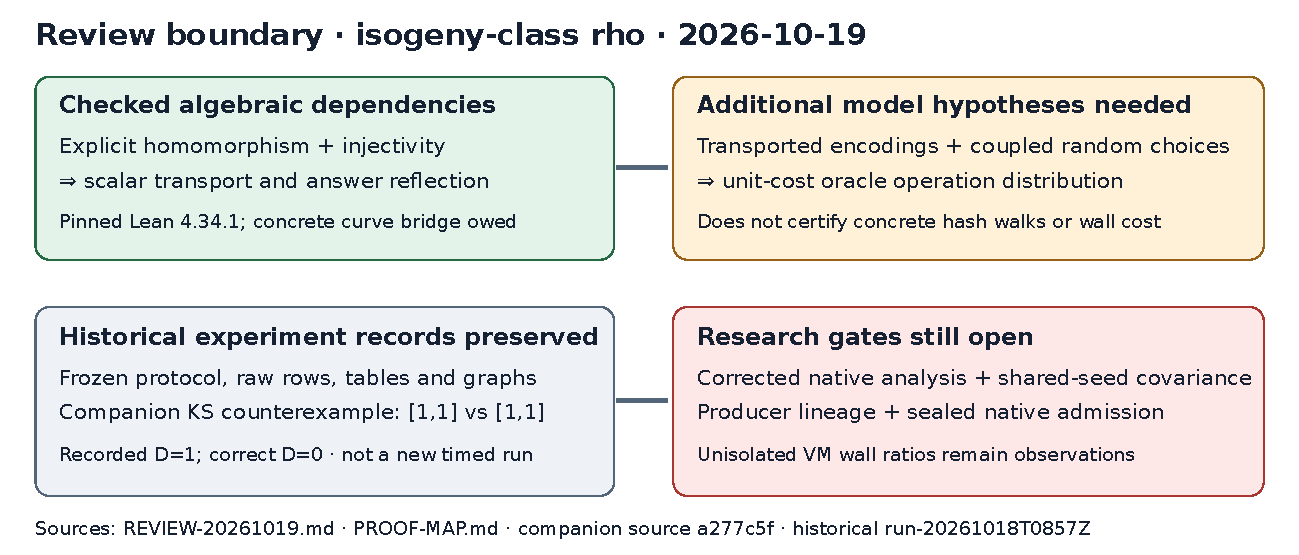
\includegraphics[width=\linewidth]{figures/review-boundary-20261019.pdf}
\caption{Review boundary. Checked algebraic dependencies do not close
the concrete-model or experiment-admission gaps. Historical statistical
figures below retain their original values and provisional inference.}
\label{fig:review-boundary}
\end{figure}

\section{Introduction}

Isogenous elliptic curves over a finite field have the same number of points,
and the isogeny class of an ordinary curve $E/\FF_q$ is large: it is a union
of endomorphism-ring strata, one for each order $\OO$ between $\ZZ[\pi]$ and
the maximal order $\OO_K$ of $K = \QQ(\pi)$, each a torsor under the class
group of $\OO$~\cite{Kohel1996,FouquetMorain2002,Sutherland2013}. It is
natural to ask whether some curve in the class is a \emph{better} place to
solve a discrete logarithm than another, and the question has two very
different answers depending on what ``solve'' means. For a \emph{generic}
algorithm in a coupled unit-cost oracle model, the transport argument is
algebraic (Section~\ref{sec:null}): an isogeny of degree prime to $n$ carries
$\langle P\rangle$ isomorphically. Injectivity of an arbitrary encoding
alone does not equate concrete hash-partitioned walks or machine costs.
For algorithms that use a curve's structure the answer
is yes in at least two known ways, both on the \emph{crater}: the
automorphisms of $j \in \{0, 1728\}$ fold rho by $\sqrt{3}$ or
$\sqrt{2}$~\cite{DuursmaGaudryMorain1999,WienerZuccherato1998}, and the
Frobenius of a Koblitz curve folds it by
$\sqrt{m}$~\cite{GallantLambertVanstone2000,WienerZuccherato1998}. Jao, Miller
and Venkatesan~\cite{JaoMillerVenkatesan2005} proved that the discrete logarithm
is random self-reducible across an isogeny class under a rapid-mixing
assumption on the isogeny graph, so an easier curve, if one existed, would
make the whole class easy.

\paragraph{Related work, and what is and is not new.} Galbraith~\cite{Galbraith1999}
showed how to construct isogenies between ordinary curves of the same order
and so transport a discrete logarithm between them; its cost for the worst
pair of curves was improved recently~\cite{Galbraith2024}, and Jao, Miller and
Venkatesan~\cite{JaoMillerVenkatesan2005} proved random self-reducibility
under conditions on the endomorphism rings. These are reductions and
algorithms for \emph{moving} an instance; they do not measure what a generic
solver costs on the far side, which is the question here. In a literature
search we found no earlier measured whole-class comparison of rho with
explicit isogenies; that is a statement about our search, not a proof that
none exists. The null itself is a short consequence of the group law and is
not offered as new. The V\'elu map on points in characteristic two
(Appendix~\ref{app:char2}) is a specialisation of V\'elu's characteristic-free
formulas~\cite{Velu1971} to one model, and we make no claim that it was
unknown; the mod-$8$ proposition of Section~\ref{sec:torsion} is elementary
and may well appear in the literature on isogenies of binary curves, where we
did not find it stated.

None of this says what a measurement would show, and a measurement is what a
claim of the form ``curve $X$ solves faster'' or ``no curve solves faster''
needs. Such claims are comparative: one number on one curve has no reference.
The historical study used a frozen protocol, a null population, planted
controls, one instrument on every arm, and preregistered decision rules.
The review identified statistical and admission gaps; those safeguards
alone do not validate the reported inference.

\paragraph{Contributions.}
\begin{enumerate}
\item A native tool, \code{isoclass-rho}, that walks the $\ell$-isogeny class
  of a curve over $\FF_p$ or $\FF_{2^m}$ over any set of primes, keyed by
  $j$-invariant, finds each $\ell$-kernel by one of three routes (Elkies'
  construction from $\Phi_\ell$; factoring the division polynomial and
  running x-only ladders in the kernel's field $\FF_{q^d}$; and, for degrees
  whose division polynomial is out of reach, a \emph{torsion route} through
  $\ell$-torsion abscissae in $\FF_{q^d}$, $d = \operatorname{ord}(\pm\lambda)$),
  pushes points through the isogeny with Kohel's normalised formula over
  $\FF_p$ and an explicit formula we derive for ordinary curves in
  characteristic two, verifies every edge on points, computes every stratum's
  class number and the exact class size, assigns each curve its
  endomorphism-ring conductor, and runs Pollard rho with negation,
  automorphism and Frobenius folds (Section~\ref{sec:tool}).
\item A preregistered controlled experiment on four isogeny classes: prime,
  $j = 0$, generic binary and Koblitz, $200$ measured curves and $85{,}425$
  solves, with isomorphic and field-basis controls, an A/A replica, two
  planted effects and three structural folds (Sections~\ref{sec:design}
  and~\ref{sec:results}).
\item A historical comparison with reported resolution of about $18\%$
  per curve, $6.5\%$ per stratum and $2\%$ class-wide. Primary class
  comparisons remained within their reported bands, while ancillary
  generator and shift comparisons include exceptions. Reported crater
  folds include $0.113$ of the plain walk on the Koblitz crater.
  These statistical conclusions are provisional pending corrected native
  analysis, covariance assessment and the admission checks described above
  (Section~\ref{sec:results}).
\item Two side results: for odd $m$ every prime of the conductor of a curve
  over $\FF_{2^m}$ is $\equiv \pm 1 \pmod 8$ (Proposition~\ref{prop:mod8}),
  together with the recorded conductor factorization $703889=409\cdot1721$
  and stated volcano hypotheses, this identifies the off-crater degrees
  of the Koblitz class over $\FF_{2^{41}}$; and the torsion route that finds such
  $409$- and $1721$-isogenies in minutes (Section~\ref{sec:torsion}).
\end{enumerate}

\paragraph{What this paper is not.} It is not an attack, not an
index-calculus result, and not a statement about any standardised curve.
Its positive effects are the well-known crater folds, measured as positive
controls. Its main content is a historical comparison whose statistical
inference and experiment admission remain under review.

\section{Algebraic transport and the generic-model boundary}
\label{sec:null}

Let $E/\FF_q$ be ordinary, $P \in E(\FF_q)$ of prime order $n$, $Q = kP$, and
$\varphi\colon E \to E'$ an $\FF_q$-rational isogeny of degree $\ell$ with
$\ell \nmid n$. Then $\varphi$ restricted to $\langle P\rangle$ is injective
(its kernel has order $\ell$), so $\varphi(P)$ has order $n$ and
$\varphi(Q) = k\,\varphi(P)$: the instance moves to $E'$ with the same
logarithm. In a \emph{generic unit-cost oracle model}, with encodings and
random choices transported through the same isomorphism, an algorithm has
the same group-operation distribution on the two presentations. This is a
model statement: injectivity alone does not identify the hash partitions of
two concrete rho implementations or their wall costs. The checked Lean
dependencies prove scalar transport and reflection of answers under explicit
homomorphism and injectivity hypotheses; the concrete curve and oracle-cost
bridges remain open (the proof map records them). For Pollard rho with an $r$-adding
walk~\cite{Pollard1978,Teske2001,vanOorschotWiener1999} the expectation is
about $\sqrt{\pi n/2}$ group operations, times roughly $1/\sqrt{1 - 1/r}$
($1.016$ at $r = 32$), and times $1/\sqrt{|G|}$ when the walk is folded by a
group $G$ of cheap maps on $\langle P\rangle$ whose orbits it canonicalises.

Concrete comparisons can additionally reflect (i) the cost of a group
operation, which depends on the coordinate representation, field and curve
coefficients; and (ii) the cheap maps a curve
admits: $\Aut(E)$ beyond $\pm 1$ at $j \in \{0, 1728\}$, and the $2$-power
Frobenius $\tau\colon (x, y) \mapsto (x^2, y^2)$ when $E$ is defined over
$\FF_2$. Both live on the crater: a curve with $\Aut(E) \ne \pm 1$ has
$\End(E) = \OO_K$ for $K = \QQ(\sqrt{-3})$ or $\QQ(\sqrt{-4})$, and a curve
whose coefficients lie in $\FF_2$ has $\End(E) \ni \tau$ with
$\ZZ[\tau] = \OO_K$ for $K = \QQ(\sqrt{-7})$. Every other curve of the class
has lost the map (its $j$ is not special; its coefficients are not in
$\FF_2$). The coupled unit-cost model preserves the transported algorithm's
operation distribution; concrete walks require separate measurement.
The historical experiment attempted that comparison, subject to the
statistical and admission limits now recorded.

\section{The tool}
\label{sec:tool}

\code{isoclass-rho} (\art{crypto:src/bin/isoclass_rho/}, about five thousand
lines of Rust, no computation in Python) has two phases. \code{walk} explores
the class and carries instances; \code{measure} runs rho on the recorded
curves. Every statistic in this paper is computed in the tool; the plotting
and tabulating scripts only lay out recorded values.

\subsection{Class arithmetic}
$\#E(\FF_q)$ is counted by baby-step giant-step on random points and checked
on eight more; $t = q + 1 - \#E$, $D = t^2 - 4q = f^2 D_K$. The class number
$h(D_K)$ is counted from reduced primitive forms; $h(d^2 D_K)$ for every
$d \mid f$ follows from the conductor formula and is cross-checked by counting
$h(f^2 D_K)$ directly (the two agreed in every class). The class size is
$\sum_{d \mid f} h(d^2 D_K)$, one curve per $\FF_q$-isomorphism class in each
stratum~\cite{Kohel1996,Sutherland2013}.

\subsection{Three routes to an $\ell$-kernel}
\label{sec:routes}
A prime $\ell$ is \emph{active} when the curve has a rational $\ell$-isogeny:
$\ell \mid f$, or $\ell \nmid f$ with $\left(\frac{D_K}{\ell}\right) = 1$.
All three routes produce the same object, the monic kernel polynomial $h$
of degree $(\ell - 1)/2$ whose roots are the abscissae of the non-trivial
kernel points.

\emph{Elkies route} ($\FF_p$, $j \notin \{0, 1728\}$). The roots of
$\Phi_\ell(j, Y)$ are the neighbours' invariants, and Elkies'
construction~\cite{Elkies1998,Schoof1995} gives $h$ from a root; $\Phi_\ell$ is
built natively from the $q$-expansion of $j$ ($\ell = 61$ takes $15$ s). At
$j \in \{0, 1728\}$ the automorphisms identify quotients of non-rational
subgroups, so the roots of $\Phi_\ell(j, Y)$ over-count; there the next route
is used.

\emph{Division route} (any field, any $j$). The $\ell$-division polynomial is
factored over $\FF_q$ into its irreducible factors of degree $d \mid
(\ell-1)/2$; a root $x(T)$ of such a factor lies in $\FF_{q^d}$, the x-only
ladder gives $x(iT)$ there, and $\langle T\rangle$ is rational exactly when
$\prod_i (x - x(iT))$ has coefficients in $\FF_q$. The kernel-field degree
$d$ is the ``hardness'' of the kernel: the smallest extension its abscissae
generate. In characteristic two we use Koblitz's recursion for
$y^2 + xy = x^3 + ax^2 + b$~\cite{Koblitz1991}, checked against
$x(3P) = x + f_2 f_4 / f_3^2$ on random points.

\emph{Torsion route} (Section~\ref{sec:torsion}), for $\ell \mid f$ at a vertex
above the floor, where the Frobenius is a scalar $\lambda$ on $E[\ell]$ and
every subgroup is rational.

\subsection{Maps on points, and verification}
Over $\FF_p$ the normalised isogeny is Kohel's~\cite{Kohel1996}
\[
X = \ell x - 2\sigma - 2(3x^2 + a)\frac{h'}{h} - 4(x^3 + ax + b)\Bigl(\frac{h'}{h}\Bigr)', \qquad Y = y\,X'(x),
\]
with $\sigma$ the sum of the roots of $h$. Over $\FF_{2^m}$, for
$E\colon y^2 + xy = x^3 + ax^2 + b$ and odd $\ell$, we specialise V\'elu's
general formulas~\cite{Velu1971,Washington2008} to $a_1 = 1$, $a_3 = a_4 = 0$:
with $L = h'/h$ and the Hasse derivatives $D_2 h$, $D_3 h$,
\begin{equation}\label{eq:char2}
X = x + xL + x^2 L^2, \qquad
Y = y + x^3 L_3 + xL + (x + y + x^2)(xL^2 + L), \qquad
L_3 = L^3 + L\,\frac{D_2 h}{h} + \frac{D_3 h}{h},
\end{equation}
onto the codomain $y^2 + xy = x^3 + ax^2 + (b + \sigma + \sigma^2)$. The
derivation (Appendix~\ref{app:char2}) uses only that in characteristic two
$\sum_Q 1/(x + x_Q)^2 = L^2$ and that the power sum $\sum_Q 1/(x + x_Q)^3$
follows from Newton's identities with the Hasse derivatives as elementary
symmetric functions. Every edge the walk uses is then verified on points:
images lie on the codomain, $\varphi(P + Q) = \varphi(P) + \varphi(Q)$, and
$n\,\varphi(P) = O \ne \varphi(P)$; $\#E$ is re-counted on every measured
curve; and every rho solve must return the planted $k$. A wrong formula
cannot survive these checks, which is how the characteristic-two map and the
torsion route were validated in the tool's self-test before any measurement.

\subsection{Levels, strata and instances}
A curve's level in the $\ell$-volcano~\cite{FouquetMorain2002} is found from
its number of rational $\ell$-kernels (one at the floor) and
non-backtracking walks from three neighbours to the floor; its conductor
relative to the walked primes is $\prod_\ell \ell^{\,\mathrm{level}_\ell}$,
which names its endomorphism-ring stratum. The root's instance $(P, kP)$ is
pushed down the breadth-first tree to every measured curve. \emph{Shifted}
instances are drawn on other source curves and carried up to the root through
dual edges (any rational isogeny back to the parent's $j$, composed with the
model isomorphism, sixth roots at $j = 0$) and down again. \emph{Generators}
are $P_i = r_i P$, $Q_i = r_i Q$ with $r_i$ uniform, the same $k$.

\subsection{Rho and its folds}
Single walker, $32$-adding walk~\cite{Teske2001}, distinguished points with
$\theta = 2^{-8}$~\cite{vanOorschotWiener1999}, restart after $40 \cdot 2^8$
distinguished-point-free steps; trial $s$ uses the same seed on every arm, and
all (arm, seed) jobs are shuffled over the threads. The walk reproduces an
earlier single-volcano tool's walk exactly. A \emph{fold} steps from the
canonical representative of a point's orbit under negation, $\Aut(E)$ at
$j \in \{0, 1728\}$, or $\langle\tau\rangle$ (with or without negation) on a
Koblitz curve, tracking the scalar; $2$-cycles are prevented by the
look-ahead rule and longer fruitless cycles are escaped deterministically from
the cycle's minimum by doubling~\cite{WienerZuccherato1998,BernsteinLangeSchwabe2011}.

\section{The torsion route, and why the Koblitz class needs it}
\label{sec:torsion}

\begin{proposition}\label{prop:mod8}
Let $E/\FF_{2^m}$ be ordinary with $m$ odd and conductor $f$, i.e.
$t^2 - 2^{m+2} = f^2 D_K$. Every odd prime $\ell \mid f$ satisfies
$\ell \equiv \pm 1 \pmod 8$.
\end{proposition}
\begin{proof}
$\ell \mid f$ implies $t^2 \equiv 2^{m+2} \pmod{\ell^2}$, so $2^{m+2} = 4 \cdot
2^m$ is a square modulo $\ell$, hence so is $2^m$, hence (as $m$ is odd) so is
$2$; and $2$ is a quadratic residue modulo an odd prime $\ell$ exactly when
$\ell \equiv \pm 1 \pmod 8$.
\end{proof}
The number-theoretic implication is checked by
\code{ConductorModEight.primeDivisorModEight} in the pinned Lean project:
for an odd prime $p$, odd $m$, $p\mid f$ and the supplied integer identity
$t^2-4\cdot2^m=f^2D$, it proves $p\bmod8\in\{1,7\}$.
It uses Mathlib's quadratic-residue characterization of $2$.
Certifying the concrete curve's $t,f,D$ and the volcano interpretation
remains a separate bridge; the theorem does not read the native records.

So a binary curve over an odd-degree field has no $3$-, $5$-, $11$- or
$13$-isogeny off any crater; the first candidates are $7, 17, 23, 31, 41, \ldots$
For the Koblitz curve $E_0\colon y^2 + xy = x^3 + 1$ over $\FF_{2^{41}}$,
$D = -7 \cdot 703889^2$ with $703889 = 409 \cdot 1721$ and $h(-7) = 1$: the
curve is alone on the crater of both volcanoes, every horizontal edge is a
loop, and the only way off the crater is a $409$- or a $1721$-isogeny
(\run\art{/K/walk.json}, \code{class}). The division polynomials have degree
$83{,}640$ and $1{,}480{,}920$, and even $\Phi_{409}$ is out of practical reach
here.

The torsion route uses the structure instead. At a vertex above the floor of
the $\ell$-volcano the Frobenius acts on $E[\ell]$ as a scalar
$\lambda \equiv t/2 \pmod \ell$, so every one of the $\ell + 1$ subgroups is
rational and the abscissae of $E[\ell]$ lie in $\FF_{q^d}$ with
$d = \operatorname{ord}(\pm\lambda)$ in $(\ZZ/\ell)^*/\pm 1$ ($d = 204$ for
$\ell = 409$, $215$ for $\ell = 1721$). We build $\FF_{q^d} = \FF_q[y]/(g)$ with
$g$ an irreducible trinomial or pentanomial over $\FF_2$ of degree $d$,
coprime to $m$ so it stays irreducible over $\FF_{2^m}$~\cite{LidlNiederreiter1997}.
A random abscissa $x \in \FF_{q^d}$ belongs to a point of $E$ or of its
quadratic twist over $\FF_{q^d}$, whose orders $q^d + 1 \mp s_d$ follow from
the Frobenius eigenvalue recurrence; the Montgomery x-only
ladder~\cite{Montgomery1987,LopezDahab1999}, which needs no $y$ and does not
distinguish a curve from its twist, by the matching cofactor gives an
$\ell$-torsion abscissa $x(T)$, checked by
$x(\tfrac{\ell+1}{2}T) = x(\tfrac{\ell-1}{2}T)$. Its multiples $x(iT)$ follow
from the differential-addition ladder, and the kernel polynomial is the
product over Frobenius orbits $\{x(\pm i\lambda^j T)\}$, each orbit's
polynomial having $\FF_q$ coefficients (a non-rational subgroup, or a wrong
$\lambda$, fails this test). One $409$-kernel costs about one minute on a
loaded core (a ladder of $8{,}347$ bits in $\FF_{2^{41\cdot 204}}$ takes $31$ s)
and one $1721$-kernel about five; the walk sampled three kernels of each
degree at each vertex above the floor ($54$ ladders in all) and found the
dual of a sampled edge by pushing a second torsion abscissa through it. Each
of the ten resulting edges passed the point checks of
Section~\ref{sec:tool}, and $\#E$ was re-counted on all eleven curves.

\section{Experimental design}
\label{sec:design}

The protocol (\art{crypto:research/isogeny-class-rho/PROTOCOL.md}, sha256
\code{81c3232b\ldots}) was frozen before the first measurement and names the
classes, the primes, the budgets, the controls, the decision rules, the
multiple-comparison correction, the power check and the pre-flight runtime.

\paragraph{Classes.} Table~\ref{tab:classes}. P1 and B1 were found by random
search for a conductor divisible by the wanted primes; P0 by a search among
$j = 0$ curves; K is the Koblitz curve $E_0$ at the first field degree in
$[23, 62]$ with a prime-order subgroup of at least $40$ bits.

\begin{table}[H]
\centering\footnotesize
\caption{The four classes. $n$ is the prime order of $\langle P\rangle$;
class size is $\sum_{d\mid f} h(d^2 D_K)$; ``measured'' counts the curves rho
ran on, ``strata'' the endomorphism-ring strata they cover. Records:
\run\art{/<class>/walk.json}.}
\label{tab:classes}
\begin{tabular}{@{}lllrrrr@{}}
\toprule
class & field; root curve & $D = f^2 D_K$ & $n$ (bits) & $h(D_K)$ & class size & measured / strata \\
\midrule
P1 & $\FF_p$, $p = 235212858169$; & $315^2\cdot(-8205107)$ & $35$ & $612$ & $347{,}004$ & $104$ / $12$ of $12$ \\
   & \quad $a = 228505936335$, $b = 82673460332$ & & & & & \\
P0 & $\FF_p$, $p = 217710133177$; & $27792^2\cdot(-3)$ & $33$ & $1$ & $38{,}472$ & $45$ / $12$ of $20$ \\
   & \quad $a = 0$, $b = 205801627284$ ($j = 0$) & & & & & \\
B1 & $\FF_{2^{37}}$, $z^{37}{+}z^6{+}z^4{+}z{+}1$; & $833^2\cdot(-660703)$ & $37$ & $296$ & $327{,}080$ & $40$ / $6$ of $6$ \\
   & \quad $a = 89938361934$, $b = 61869205585$ & & & & & \\
K  & $\FF_{2^{41}}$, $z^{41}{+}z^3{+}1$; & $703889^2\cdot(-7)$ & $40$ & $1$ & $708{,}153$ & $11$ / $4$ of $4$ \\
   & \quad $y^2 + xy = x^3 + 1$ & & & & & \\
\bottomrule
\end{tabular}
\end{table}

\paragraph{Primes walked.} P1: $\ell \in \{2, \ldots, 19\}$ everywhere and
$\{23, \ldots, 61\}$ at the first three vertices (the horizontal ``hard''
edges, with kernel fields up to $\FF_{p^{23}}$); $3$ ($2$ levels), $5$, $7$
($1$ level each) are its volcano primes. P0: $\{2, 3, 5, 7, 11, 13\}$
(volcanoes of depth $4$ and $2$; the prime $193$ of its conductor was not
walked). B1: $\{7, 17\}$ everywhere ($7$ of depth $2$, $17$ of depth $1$),
$\{23, 31\}$ at the first three vertices. K: $\{409, 1721\}$ by the torsion
route. Inert primes with $\ell \nmid f$ were recorded as inactive.

\paragraph{Measured set.} The root, up to eight curves per stratum spread
over the breadth-first order, and the curves reached through the largest
degrees. The root's instance was carried to each.

\paragraph{Modes and budgets.} \emph{Class}: every measured curve $\times$
$100$ paired seeds, plus three isomorphic models of the root
($\FF_p$: $(u^4 a, u^6 b)$; $\FF_{2^m}$: the same curve in three other
polynomial bases of the field, since $y \mapsto y + sx$ leaves every abscissa
and hence the walk unchanged), an A/A replica of the root under an
independent seed set, a planted negation fold (expected $0.707$), a planted
$4$-adding walk (Teske's heuristic $\sqrt{1 - 1/32}/\sqrt{1 - 1/4} = 1.137$),
and the structural folds where the root admits them. \emph{Generators}:
$6$/$4$/$6$/$3$ curves $\times$ $100$/$100$/$64$/$64$ generators $\times$ $25$
seeds. \emph{Shift}: $5$/$4$/$5$/$3$ sources $\times$ every measured curve
$\times$ $25$ seeds.

\paragraph{Decision rules.} R1: a curve against the pooled solves of the
others by Welch's $z$, family $m$ = number of curves, $\alpha = 0.05$,
threshold $z_{\mathrm{crit}}$ at $\alpha/m$ two-sided; R2: Kruskal--Wallis
and one-way ANOVA across curves with the between-curve variance ratio
$\operatorname{var}(\text{arm means})/(\text{pooled var}/T)$, heterogeneity
``detected'' if $p < 0.05$; R3: the same for pooled strata, levels,
distances, parent degrees and kernel-field degrees; R4: the planted
negation fold's interval must exclude $1$ and the structural folds must lie
within $15\%$ of $1/\sqrt{|G|}$, else every null verdict of that class is
inconclusive; R5: per curve, Kruskal--Wallis across generators, the variance
ratio, Bonferroni-flagged generators and Spearman correlations of the
generator mean with $r$, $\mathrm{bits}(r)$, $\mathrm{popcount}(r)$ and
$x(P_i)$; R6: Kruskal--Wallis by target and by source and $\eta^2$ of each
factor. Verdict wording is fixed: ``within the control distribution'' or
``more extreme than the family''. Power: with a single-solve coefficient of
variation of $0.52$, $T = 100$ gives a per-curve mean with $5.2\%$ standard
error, so a per-curve effect of about $18\%$ is detectable at $m \approx 100$,
a stratum effect of about $6.5\%$, a class-wide shift of about $2\%$; the
strong plant ($29\%$) should be seen per arm at $|z| \approx 5.6$, the weak
plant ($14\%$) near the threshold.

\paragraph{Execution.} The walks were run from a frozen command card by a
separate executor; the measurements by the author's session; every command,
log and record is in the run directory. Each class mode was replayed at five
seeds afterwards and reproduced the recorded iteration counts exactly
($550/550$, $260/260$, $230/230$, $95/95$ rows). Wall times come from a shared
four-vCPU virtual machine with other jobs running and are indicative only;
group operations are the unit of every comparison.

\section{Results}
\label{sec:results}

\subsection{Every curve, stratum and route}

\begin{table}[H]
\centering\footnotesize
\caption{Class mode: $100$ paired seeds per arm, all solves correct. ``ratio''
is the pooled mean over $\sqrt{\pi n/2}$ ($\times 1.016$ expected for the
$32$-adding walk); $|z|_{\max}$ is the largest Welch $z$ of a measured curve
against the pooled others, with the Bonferroni threshold; VR is the
between-curve variance ratio. Records: \run\art{/<class>/class/results.json}.}
\label{tab:class}
\begin{tabular}{@{}lrrrrrrrrr@{}}
\toprule
class & curves & solves & $\sqrt{\pi n/2}$ & pooled mean & ratio & $|z|_{\max}$ / $z_{\mathrm{crit}}$ & KW $p$ & ANOVA $p$ & VR \\
\midrule
P1 & $104$ & $10{,}400$ & $202{,}614$ & $206{,}675$ & $1.020$ & $3.03$ / $3.49$ & $0.089$ & $0.101$ & $1.18$ \\
P0 & $45$ & $4{,}500$ & $110{,}515$ & $110{,}942$ & $1.004$ & $2.42$ / $3.26$ & $0.162$ & $0.264$ & $1.13$ \\
B1 & $40$ & $4{,}000$ & $328{,}549$ & $334{,}995$ & $1.020$ & $3.02$ / $3.23$ & $0.158$ & $0.292$ & $1.11$ \\
K & $11$ & $1{,}100$ & $929{,}277$ & $924{,}231$ & $0.995$ & $2.38$ / $2.84$ & $0.209$ & $0.076$ & $1.70$ \\
\bottomrule
\end{tabular}
\end{table}

In every class every measured curve is within the control distribution
(Table~\ref{tab:class}), and no across-curve test detects heterogeneity. The
pooled distributions are the familiar rho shape: for P1, minimum $2{,}082$,
median $193{,}529$, maximum $705{,}972$ operations, coefficient of variation
$0.52$, skewness $0.64$. The spread of curve means is $1.1$ to $1.7$ times
what the pooled single-solve spread predicts ($11{,}751$ against $10{,}814$ on
P1; $62{,}858$ against $48{,}378$ on K's eleven curves), the largest ratio on
the smallest family and carried by no single curve. Per-step cost is flat
within a class ($429$--$523$ ns per operation across P1's $104$ curves,
$528$--$600$ ns across B1's $40$).

\begin{table}[H]
\centering\footnotesize
\caption{P1 pooled by endomorphism-ring stratum: conductor $f_v$ of
$\End(E_v)$ relative to $\OO_K$, the stratum's class number $h(f_v^2 D_K)$
(how many curves share that ring), eight measured curves each, $800$ solves.
Record: \run\art{/P1/class/results.json}, \code{groups}.}
\label{tab:strata}
\begin{tabular}{@{}rrrrr@{}}
\toprule
$f_v$ & $h(f_v^2 D_K)$ & mean $\pm$ 95\% CI & ratio & $z$ vs rest \\
\midrule
$1$ (crater) & $612$ & $212{,}144 \pm 7{,}338$ & $1.047$ & $1.52$ \\
$3$ & $1{,}224$ & $206{,}365 \pm 5{,}391$ & $1.019$ & $-0.12$ \\
$5$ & $3{,}672$ & $206{,}804 \pm 7{,}578$ & $1.021$ & $0.03$ \\
$7$ & $4{,}896$ & $208{,}763 \pm 7{,}647$ & $1.030$ & $0.56$ \\
$9$ & $3{,}672$ & $212{,}672 \pm 7{,}651$ & $1.050$ & $1.60$ \\
$15$ & $7{,}344$ & $208{,}215 \pm 7{,}594$ & $1.028$ & $0.41$ \\
$21$ & $9{,}792$ & $201{,}608 \pm 7{,}458$ & $0.995$ & $-1.39$ \\
$35$ & $29{,}376$ & $201{,}269 \pm 7{,}395$ & $0.993$ & $-1.49$ \\
$45$ & $22{,}032$ & $200{,}839 \pm 7{,}461$ & $0.991$ & $-1.60$ \\
$63$ & $29{,}376$ & $204{,}788 \pm 7{,}453$ & $1.011$ & $-0.52$ \\
$105$ & $58{,}752$ & $206{,}945 \pm 7{,}220$ & $1.021$ & $0.08$ \\
$315$ (floor) & $176{,}256$ & $209{,}999 \pm 7{,}352$ & $1.036$ & $0.92$ \\
\bottomrule
\end{tabular}
\end{table}

Table~\ref{tab:strata} shows the twelve strata of P1, from the crater
($\End = \OO_K$, $612$ curves) to the floor ($\End = \ZZ[\pi]$, $176{,}256$
curves): all within $\pm 5\%$ of the reference with $|z| \le 1.6$. The same
holds for every level of every volcano in every class, for the distance
from the root, for the degree of the edge that reached the curve
($3$ to $61$ on P1, $7$ to $31$ on B1, $409$ and $1721$ on K) and for the
kernel-field degree ($1$ to $23$ on P1, $3$ to $11$ on B1, $204$ and $215$ on
K); the curves reached through P1's hard horizontal isogenies have ratios
$0.88$--$1.09$ with $|z| \le 3.0$, B1's $23$- and $31$-isogeny targets
$0.92$--$1.09$, and K's four strata $0.996$ (the Koblitz crater), $1.009$,
$1.001$ and $0.978$ ($|z| \le 0.8$). The curves on the far side of a
$1721$-isogeny cost what the Koblitz curve costs.

\subsection{Controls, planted effects and the crater folds}

\begin{table}[H]
\centering\footnotesize
\caption{Control and fold arms on each root ($100$ seeds): mean ratio to
$\sqrt{\pi n/2}$ with the bootstrap 95\% interval, Welch $z$ against the
class's pooled isogenous solves, and mean wall time per solve. Isomorphic
controls are three $(u^4 a, u^6 b)$ models (P1, P0) or three other field
bases (B1, K). Records: \run\art{/<class>/class/results.json}.}
\label{tab:controls}
\begin{tabular}{@{}llrlrr@{}}
\toprule
class & arm & expected & ratio [95\% CI] & $z$ & ms / solve \\
\midrule
P1 & iso controls & $1$ & $1.158\,[1.059, 1.268]$; $1.076$; $1.052$ & $2.58$; $1.00$; $0.54$ & $104$--$114$ \\
P1 & A/A replica & $1$ & $1.053\,[0.967, 1.148]$ & $0.70$ & $103$ \\
P1 & plant: negation fold & $0.707$ & $0.725\,[0.651, 0.804]$ & $-7.45$ & $77$ \\
P1 & plant: $4$-adding walk & $1.137$ & $1.298\,[1.172, 1.440]$ & $4.03$ & $122$ \\
\midrule
P0 & iso controls & $1$ & $1.067$; $1.054$; $1.023$ & $1.17$; $0.87$; $0.40$ & $53$--$58$ \\
P0 & A/A replica & $1$ & $0.964\,[0.878, 1.059]$ & $-0.83$ & $52$ \\
P0 & plant: negation fold & $0.707$ & $0.634\,[0.567, 0.709]$ & $-9.98$ & $36$ \\
P0 & plant: $4$-adding walk & $1.137$ & $1.265\,[1.136, 1.411]$ & $3.67$ & $62$ \\
P0 & \textbf{fold: $\Aut$ of $j = 0$} & $1/\sqrt{6} = 0.408$ & $\mathbf{0.439\,[0.401, 0.481]}$ & $-25.3$ & $26$ \\
\midrule
B1 & basis controls & $1$ & $1.043$; $0.897$; $1.039$ & $0.47$; $-2.55$; $0.35$ & $174$--$199$ \\
B1 & A/A replica & $1$ & $1.161\,[1.049, 1.285]$ & $2.23$ & $217$ \\
B1 & plant: negation fold & $0.707$ & $0.771\,[0.702, 0.847]$ & $-6.40$ & $147$ \\
B1 & plant: $4$-adding walk & $1.137$ & $1.300\,[1.177, 1.435]$ & $4.20$ & $256$ \\
\midrule
K & basis controls & $1$ & $0.983$; $1.029$; $0.963$ & $-0.20$; $0.61$; $-0.55$ & $457$--$625$ \\
K & A/A replica & $1$ & $0.970\,[0.875, 1.078]$ & $-0.45$ & $456$ \\
K & plant: negation fold & $0.707$ & $0.769\,[0.705, 0.838]$ & $-5.92$ & $375$ \\
K & plant: $4$-adding walk & $1.137$ & $1.358\,[1.221, 1.508]$ & $4.74$ & $650$ \\
K & \textbf{fold: Frobenius $\tau$} & $1/\sqrt{41} = 0.156$ & $\mathbf{0.155\,[0.141, 0.170]}$ & $-48.2$ & $275$ \\
K & \textbf{fold: $\tau$ and negation} & $1/\sqrt{82} = 0.110$ & $\mathbf{0.113\,[0.103, 0.124]}$ & $-53.1$ & $212$ \\
\bottomrule
\end{tabular}
\end{table}

Table~\ref{tab:controls} is the calibration. The isomorphic and field-basis
controls and the A/A replicas sit inside the band ($|z| \le 2.6$): a change of
coordinates or of seeds moves a $100$-seed mean exactly as much as any
isogenous curve does, which is the point of the null population. The
planted negation fold is detected in every class at $|z|$ between $6$ and
$10$, and the planted $4$-adding walk at $|z| \approx 4$; the latter comes out
larger ($1.27$--$1.36$) than Teske's $1/\sqrt{1 - 1/r}$ heuristic predicts for
$r = 4$, as a walk that far from random should. The structural folds come
out where theory puts them: the order-$6$ automorphism fold on the $j = 0$
crater at $0.439$ against $0.408$ (within the $15\%$ tolerance of R4), the
Frobenius fold on the Koblitz crater at $0.155$ against $0.156$ and, with
negation, $0.113$ against $0.110$. The Koblitz folds cost $1.92$ and
$2.05$\,\textmu s per step against $0.50$ (forty-one squarings to find the
orbit's minimum), with recorded wall means of $275$ and $212$ ms per solve
against $459$ ms. These shared-VM observations were not isolated and are not
admitted wall-performance results. Neither fold exists on any other measured
curve of its class:
$\Aut = \pm 1$ away from $j = 0$, and $\tau$ is an endomorphism only when the
curve is defined over $\FF_2$, which only the crater curve is. The plain walk
costs the same on all of them.

\subsection{Generators and source curves}

On P1, $100$ generators of $\langle P\rangle$ on each of six curves with the
same secret, $25$ seeds each ($15{,}000$ solves): the standard deviation of
the $100$ generator means is $19{,}852$--$21{,}863$ against $21{,}275$--$21{,}873$
expected from the single-solve spread (variance ratios $0.84$--$1.04$),
Kruskal--Wallis $p$ between $0.44$ and $0.92$ per curve, no generator beyond
the threshold (family $600$, largest $|z|$ $3.76$ against $3.93$), and every
Spearman correlation of the generator mean with $r$, $\mathrm{bits}(r)$,
$\mathrm{popcount}(r)$ or $x(P_i)$ has $|\rho| \le 0.12$. P0 ($400$
generators), B1 ($384$) and K ($192$) read the same (variance ratios
$0.81$--$1.26$ per curve), with one cell of $384$ on B1 beyond the band on the
low side ($0.677$ $[0.535, 0.829]$ at $25$ seeds, Mann--Whitney $z = -3.3$),
the low tail of $384$ small means and not repeated by that curve's other $63$
generators or by its features. The original all-arm B1 generator
Kruskal--Wallis result is $p=0.039$. These are recorded exceptions, not
grounds for a categorical claim that the generator cannot matter; their
interpretation awaits the corrected native analysis described above.

Instances drawn on five source curves of P1 (the root and four others) and
carried to all $104$ targets, $25$ seeds per cell ($13{,}000$ solves): the
two-way decomposition gives $\eta^2 = 0.0085$ for the target and $0.0002$ for
the source, Kruskal--Wallis $p = 0.19$ by target and $0.37$ by source, and
the five sources' pooled means are $1.007$--$1.029$ of the reference. Two of
the $520$ cells lie beyond the Bonferroni band on the low side; both targets
are unremarkable in the other four rows and in the class mode ($1.013$,
$1.036$). P0 also has one flagged cell of $180$; B1 and K have no flagged
shift cell in the original report
($\eta^2_{\mathrm{source}} \le 0.0012$ everywhere). The flags and the
shared-seed covariance must be retained in a corrected analysis before
inferring source independence.

\subsection{Historical end-to-end costs}

Carrying an instance to a curve costs the isogenies on the way. The following
are historical, unisolated wall observations, not an admitted end-to-end
comparison. On P1 the Elkies edges cost $0.6$ ms ($\ell = 3$)
to $5.5$ s ($\ell = 61$, dominated by building $\Phi_{61}$ once) and a solve
$98$ ms; the transport to any measured curve was under $74$ ms. On B1 the
$23$- and $31$-isogenies cost $1.3$--$2.4$ s each by the division route
against a $0.19$ s solve. On K the $409$- and $1721$-isogenies cost $197$ s
and $978$ s per three-kernel search, so the transport to a conductor-$703889$
curve is nine to fifteen minutes against a $0.46$ s solve. The $3$D heat maps
of the run (Figures~\ref{fig:p1-3d} and~\ref{fig:k-3d}) colour each measured
curve by its mean operations and by its mean end-to-end time; the first is
flat, the second is a map of the transport.

\begin{figure}[H]
\centering
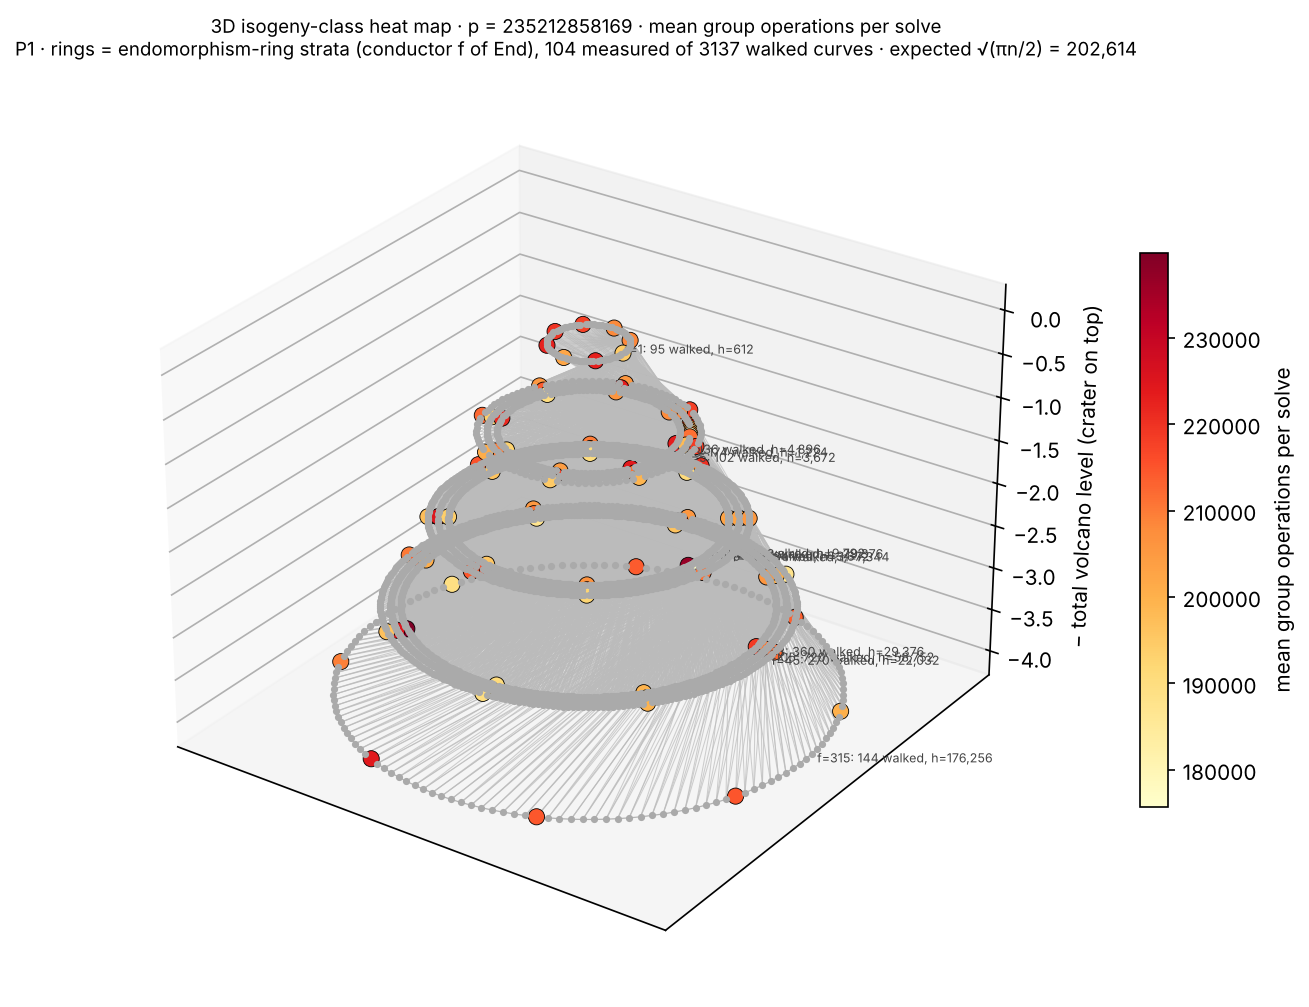
\includegraphics[width=0.49\textwidth]{figures/p1-volcano3d-ops.png}\hfill
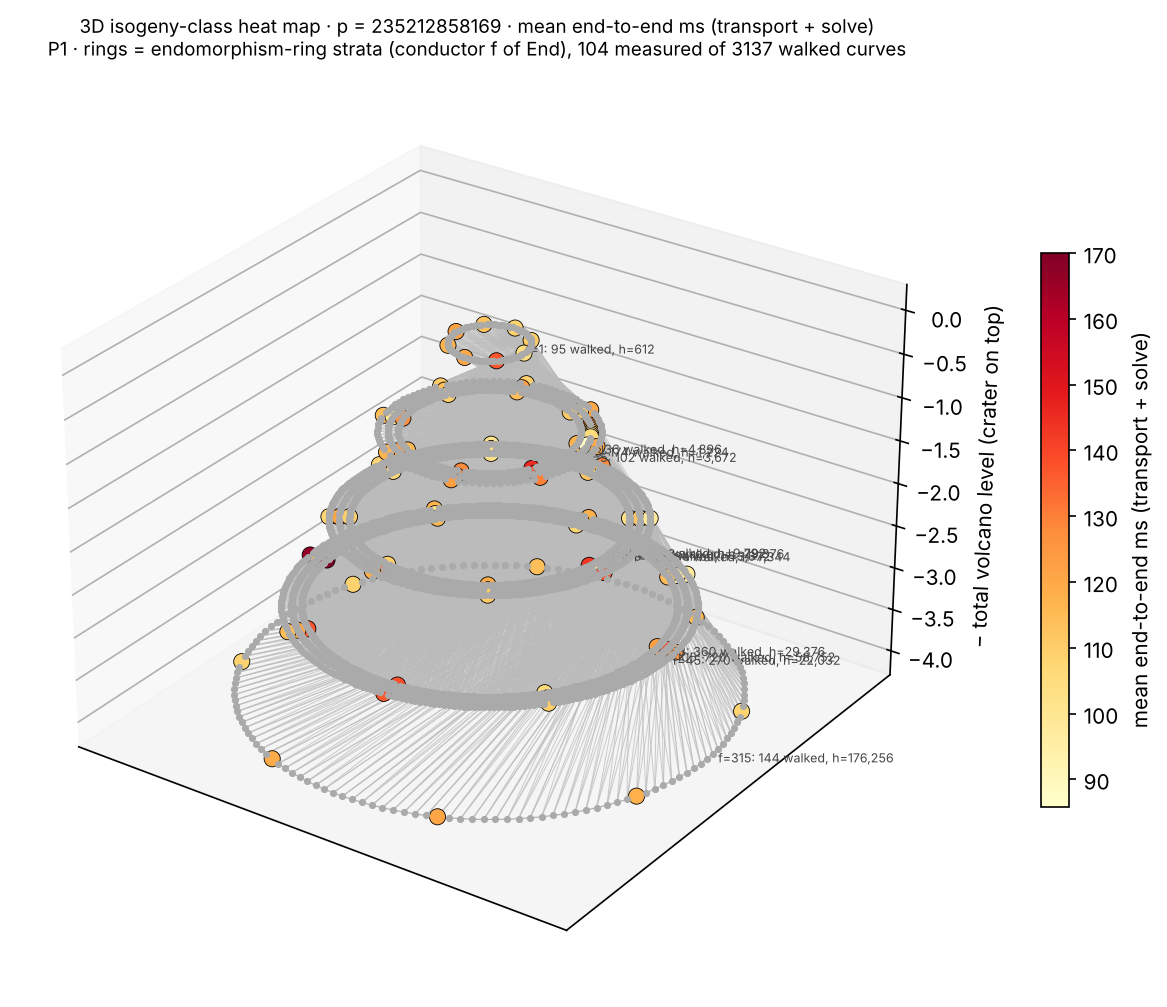
\includegraphics[width=0.49\textwidth]{figures/p1-volcano3d-e2e.png}
\caption{P1: the $3{,}137$ walked curves on their endomorphism-ring strata
(rings, crater on top, with each stratum's class number), the $104$ measured
ones coloured by mean group operations (left) and by mean end-to-end time,
transport plus solve (right). Record: \run\art{/P1/}.}
\label{fig:p1-3d}
\end{figure}

\begin{figure}[H]
\centering
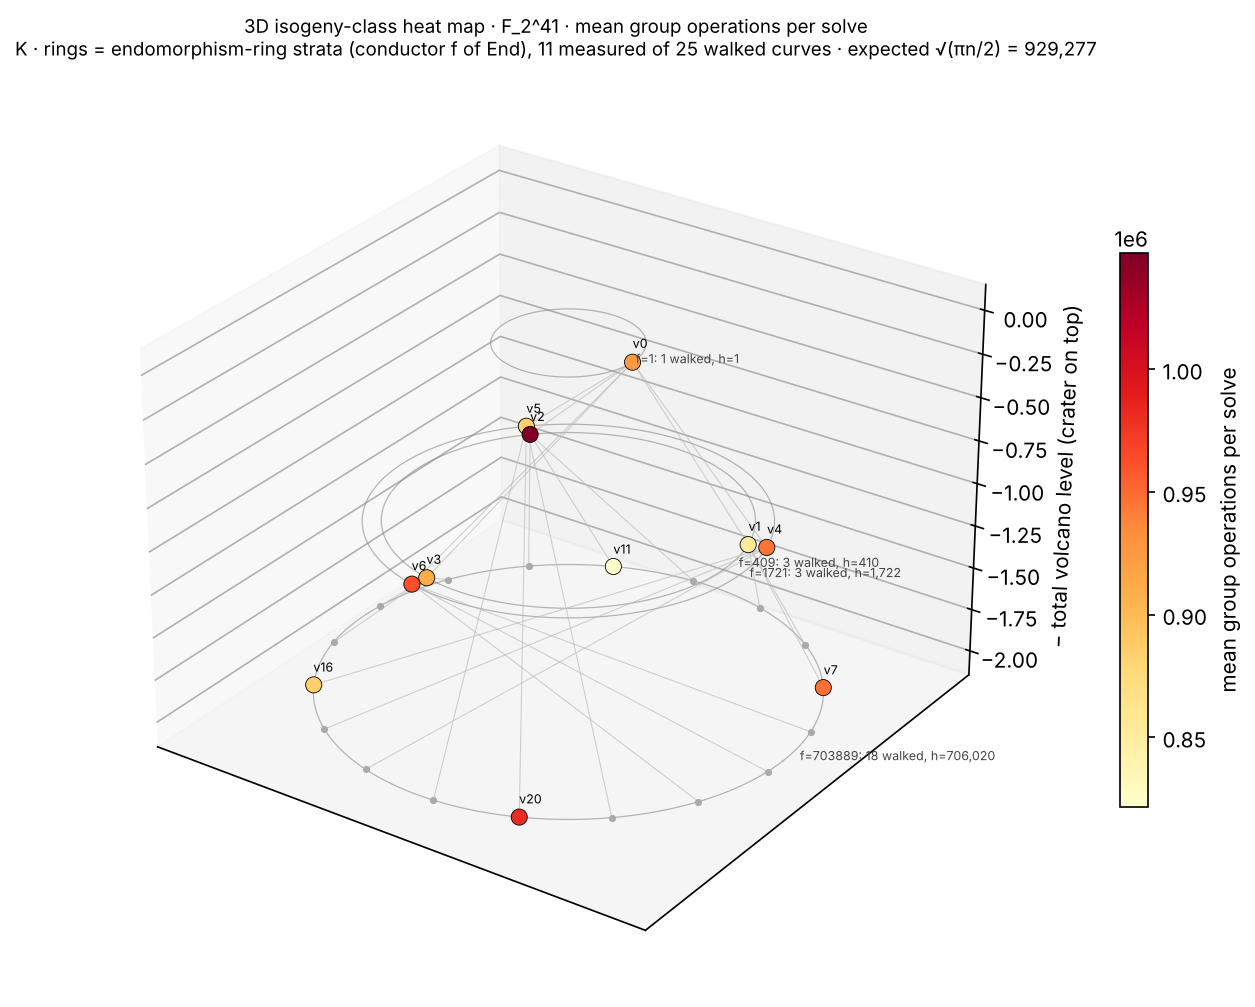
\includegraphics[width=0.62\textwidth]{figures/k-volcano3d-ops.png}
\caption{K: the Koblitz crater, its $409$- and $1721$-strata and the
conductor-$703889$ stratum of $706{,}020$ curves; $11$ measured of $25$
walked, coloured by mean operations. Record: \run\art{/K/}.}
\label{fig:k-3d}
\end{figure}

\begin{figure}[H]
\centering
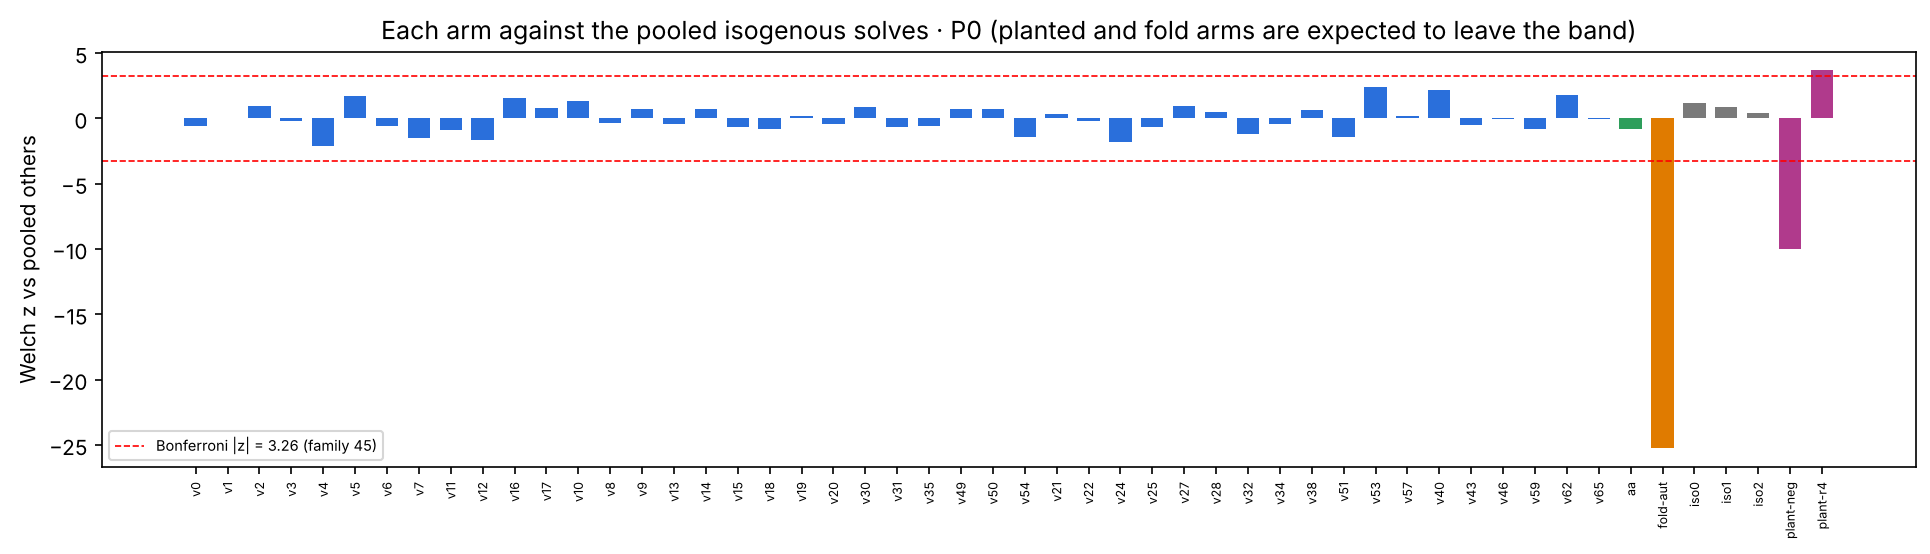
\includegraphics[width=\textwidth]{figures/p0-z-scores.png}\\[4pt]
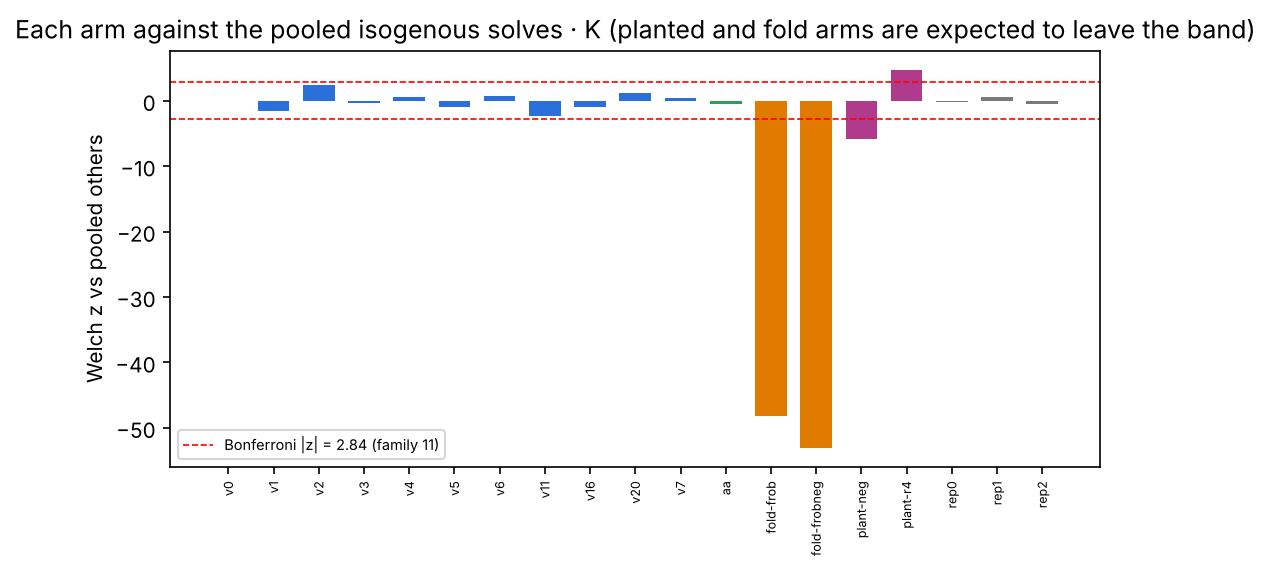
\includegraphics[width=\textwidth]{figures/k-z-scores.png}
\caption{Each arm against the pooled isogenous solves, P0 (top) and K
(bottom): every curve and control inside the Bonferroni band, the planted
and structural folds outside it. Records: \run\art{/P0/}, \run\art{/K/}.}
\label{fig:z}
\end{figure}

\section{Discussion}

\paragraph{What the record says.} The historical primary class-mode
comparisons stayed within their reported per-curve bands and detected the
planted and structural controls. Ancillary generator and source--target
flags remain visible above. Tied-sample inference, shared-seed covariance,
native-harness admission and concrete proof bridges are unresolved, so this
draft does not promote the historical analysis to a general empirical
invariance conclusion. Random self-reducibility~\cite{JaoMillerVenkatesan2005}
is the cited theoretical context, not a substitute for those gates.

\paragraph{What it does not say.} It does not say that no curve of a class
is easier for some non-generic method; index calculus on a curve with a
convenient model, or a transfer to another group, is not a generic walk and
is not measured here. It does not bound effects below the stated resolution.
It does not speak about curves outside these four classes or at
cryptographic sizes, where the only extrapolation we would make is the
theorem of Section~\ref{sec:null}. And the folds are not ``isogeny
speed-ups'': they are the crater curve's own endomorphisms, which an isogeny
takes away.

\paragraph{Hard isogenies.} The Koblitz class is the instructive case. Its
reachable off-crater neighbours are at degrees $409$ and $1721$ because the
recorded conductor is $703889=409\cdot1721$ with the stated volcano-edge
conditions. Proposition~\ref{prop:mod8} restricts prime residues but alone
does not rule out all smaller primes, such as $7$ or $17$. Division polynomials of
degree $10^5$--$10^6$ put the naive route out of reach; the torsion route
reaches them in minutes because above the floor the Frobenius is a scalar and
the kernel field is as small as $\operatorname{ord}(\pm\lambda)$ allows. The
curves on the far side are generic curves over $\FF_{2^{41}}$ with the
Koblitz curve's group and none of its structure: in practice, a $1721$-isogeny
is a way to turn a Koblitz instance into a non-Koblitz one, and nothing else.

\paragraph{Classification.} In the vocabulary of the companion repository this
is a historical bounded comparison with reported positive controls and
provisional inference, rho against rho on one instrument. It is not a
change to any index-calculus baseline and is not a
speed-up claim.

\section{Reproducibility}

Everything is in the companion repository: the tool
(\art{crypto:src/bin/isoclass_rho/}, with a self-test that checks every formula
of Section~\ref{sec:tool} against direct computation, including the
characteristic-two map, the torsion route against the division route and the
duals), the frozen protocol, the command card, every walk record (models,
levels, conductors, kernel polynomials, carried instances, transport costs),
every per-solve row (arm, seed, iterations, restarts, distinguished points,
escapes, wall time), the per-arm summaries and tests, the replays, the
figures and the report. The run is
\run; the study README is \art{crypto:research/isogeny-class-rho/README.md}.
The library's test suite ($4{,}380$ tests) passes at the commit of the run.

\appendix
\section{The characteristic-two map on points}
\label{app:char2}

V\'elu's formulas for a general Weierstrass model and a finite subgroup
$C$~\cite{Velu1971,Washington2008}, with $S$ a set of representatives of
$(C \setminus \{O\})/\pm$ and no $2$-torsion in $C$, read
$X = x + \sum_{Q\in S} \bigl[v_Q/(x - x_Q) + u_Q/(x - x_Q)^2\bigr]$ and
$Y = y - \sum_{Q \in S}\bigl[u_Q(2y + a_1 x + a_3)/(x - x_Q)^3 + v_Q(a_1(x - x_Q)
+ y - y_Q)/(x - x_Q)^2 + (a_1 u_Q - g^x_Q g^y_Q)/(x - x_Q)^2\bigr]$ with
$g^x_Q = 3x_Q^2 + 2a_2 x_Q + a_4 - a_1 y_Q$, $g^y_Q = -2y_Q - a_1 x_Q - a_3$,
$v_Q = 2g^x_Q - a_1 g^y_Q$, $u_Q = (g^y_Q)^2$, onto
$A_4 = a_4 - 5v$, $A_6 = a_6 - (a_1^2 + 4a_2)v - 7w$, $v = \sum v_Q$,
$w = \sum (u_Q + x_Q v_Q)$. For $y^2 + xy = x^3 + ax^2 + b$ in characteristic
two: $g^x_Q = x_Q^2 + y_Q$, $g^y_Q = x_Q$, $v_Q = x_Q$, $u_Q = x_Q^2$,
$w = 0$, so $A_4 = v = \sigma$ and $A_6 = b + \sigma$; the substitution
$Y \mapsto Y + \sigma$ removes the $A_4$ term and gives the codomain
$y^2 + xy = x^3 + ax^2 + (b + \sigma + \sigma^2)$. In $X$, with $u = x + x_Q$,
$x_Q/u = 1 + x/u$ and $x_Q^2/u^2 = (x_Q/u)^2$, so
$X = x + d' + xL + d'^2 + x^2 L^2 = x + xL + x^2L^2$ since $d' + d'^2$ is even,
where $L = \sum 1/u = h'/h$ and $\sum 1/u^2 = L^2$ in characteristic two. In
$Y$ the representative $y_Q$ cancels (replacing $y_Q$ by $y_Q + x_Q$ adds
$2x_Q^2/u^2 = 0$), the terms reduce to $y + \sum\bigl[x^3/u^3 + x/u\bigr] +
(x + y + x^2)\sum\bigl[x/u^2 + 1/u\bigr] + \sum x_Q$, and the final shift
$Y \mapsto Y + \sigma$ cancels the $\sum x_Q = \sigma$. The remaining power
sum $L_3 = \sum 1/u^3$ follows from Newton's identities, $p_3 = e_1 p_2 +
e_2 p_1 + e_3$ in characteristic two, with $e_k = D_k h / h$ the Hasse
derivatives (the coefficients of $h(x + T)/h(x)$), giving
$L_3 = L^3 + L\,D_2h/h + D_3h/h$ and formula~\eqref{eq:char2}. The formula is
checked in the tool's self-test by the homomorphism, codomain and order tests
on random points for $\ell \in \{3, 5, 7, 11, 13\}$ on Koblitz and generic
binary curves, and in the run by the same tests on all $533$ binary edges.

\bibliographystyle{plain}
\bibliography{refs}

\end{document}
